\subsection{K-Means}
\label{sec:ctm-km}

The first clustering algorithm we tried was K-Means \cite{macqueen1967some}. It iteratively tries to group unlabeled data points with similar features together by minimizing the mean distance between each point in each group. Figure~\ref{fig:ctm-km} visualizes the groups labeled by the K-Means algorithm on the 2017 class for the Non-Blocking IO assignment.

The K-Means algorithm constructs each group to minimize the average distance from the group's centroid to every point in its corresponding group. Since the majority of students in our data set received full marks, we assumed the majority of the data points in each group should also represent full-mark solutions. As a result, the volume of full-mark solution points should draw the centroid of each group towards \textquote{regions} representing higher marks. Based on this idea, we calculated a student's score based on their distance to their corresponding group's centroid; the closer a student was to their group's centroid, the higher their probability of receiving a high score.

Let $P_i$ denote the point representing student $i$ and $C_i$ denote the centroid of the student's group. The distance from centroid $d_i$ is defined as:
\begin{equation*}
d_i = \norm{P_i - C_i}
\end{equation*}

As mentioned in Figure~\ref{fig:ctm-km}, the scales in the axes have no tangible interpretations. Therefore, the distances from centroid $d_i$ we calculated for each point also had no meaningful interpretation. As a result, we tried to evaluate each point's centroid distance relative to all other points. In other words, we calculated each student's score based on their performance relative to the rest of their class.

Let $\mu$ denote the mean and $\sigma$ denote the standard deviation of centroid distances of every student. We calculated student $i$'s score as follows:
\begin{equation*}
\text{Score}_i = 100 - 20 \cdot \frac{\abs{d_i - \mu}}{\sigma}
\end{equation*}

This equation deducted up to 20 points for each standard deviation of centroid distance a student was from their corresponding group's centroid. We chose to deduct 20 points per standard deviation arbitrarily after experimenting with different values. The main idea was to deduct marks based on how far the solution was from the centroid, where we assumed majority of the full mark solutions were located.

\begin{figure}
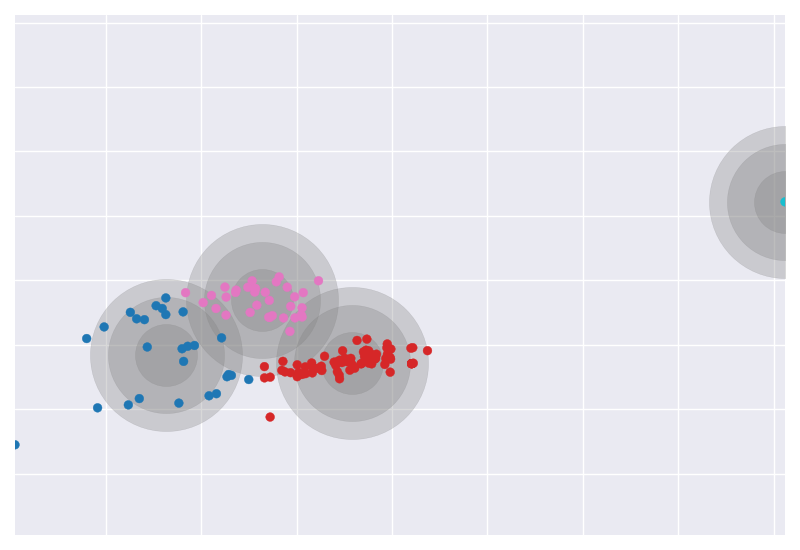
\includegraphics[width=\textwidth]{conversion-to-mark/marking_paster_nbio_ece459-a1-w2017_km}
\caption[K-Means Clustering]{Each data point represents a student solution to the Non-Blocking IO assignment from the 2017 class. It is important to note that this is a 2D projection of a multidimensional data set. Since we preprocessed the data with PCA, the first two dimensions presented here already capture the majority of the data variance. The scales in the axes are omitted because they have no tangible interpretations; they are meant for interpreting relative distances. The K-Means algorithm assigned each point a group, represented by their corresponding colour. Each set of concentric circles represent an arbitrary distance from the centroid of each group.}
\label{fig:ctm-km}
\end{figure}
